\section{Game}
In \secref{processweek2} we mentioned that main functionality of the game interface is drag and drop. during the early stages of project we created a simple prototype of the game's interface. We had different views on whether the game should be a top-down perspective or side-scrolling. We decided on the side-scrolling perspective since it was easier to perform drag and drop actions.

\todo{This section describes the design choices made in our game.}
\subsection*{Game prototype}
%hvis billedet af prototypen, beskriv hvad Tove godt kunne lide, og hvad der kunne ændres, samt tilføjet. (fløjten, ingen musik, no fancy colors on objects)
\todo{insert picture of the prototype}
\begin{figure}[H]
\centering
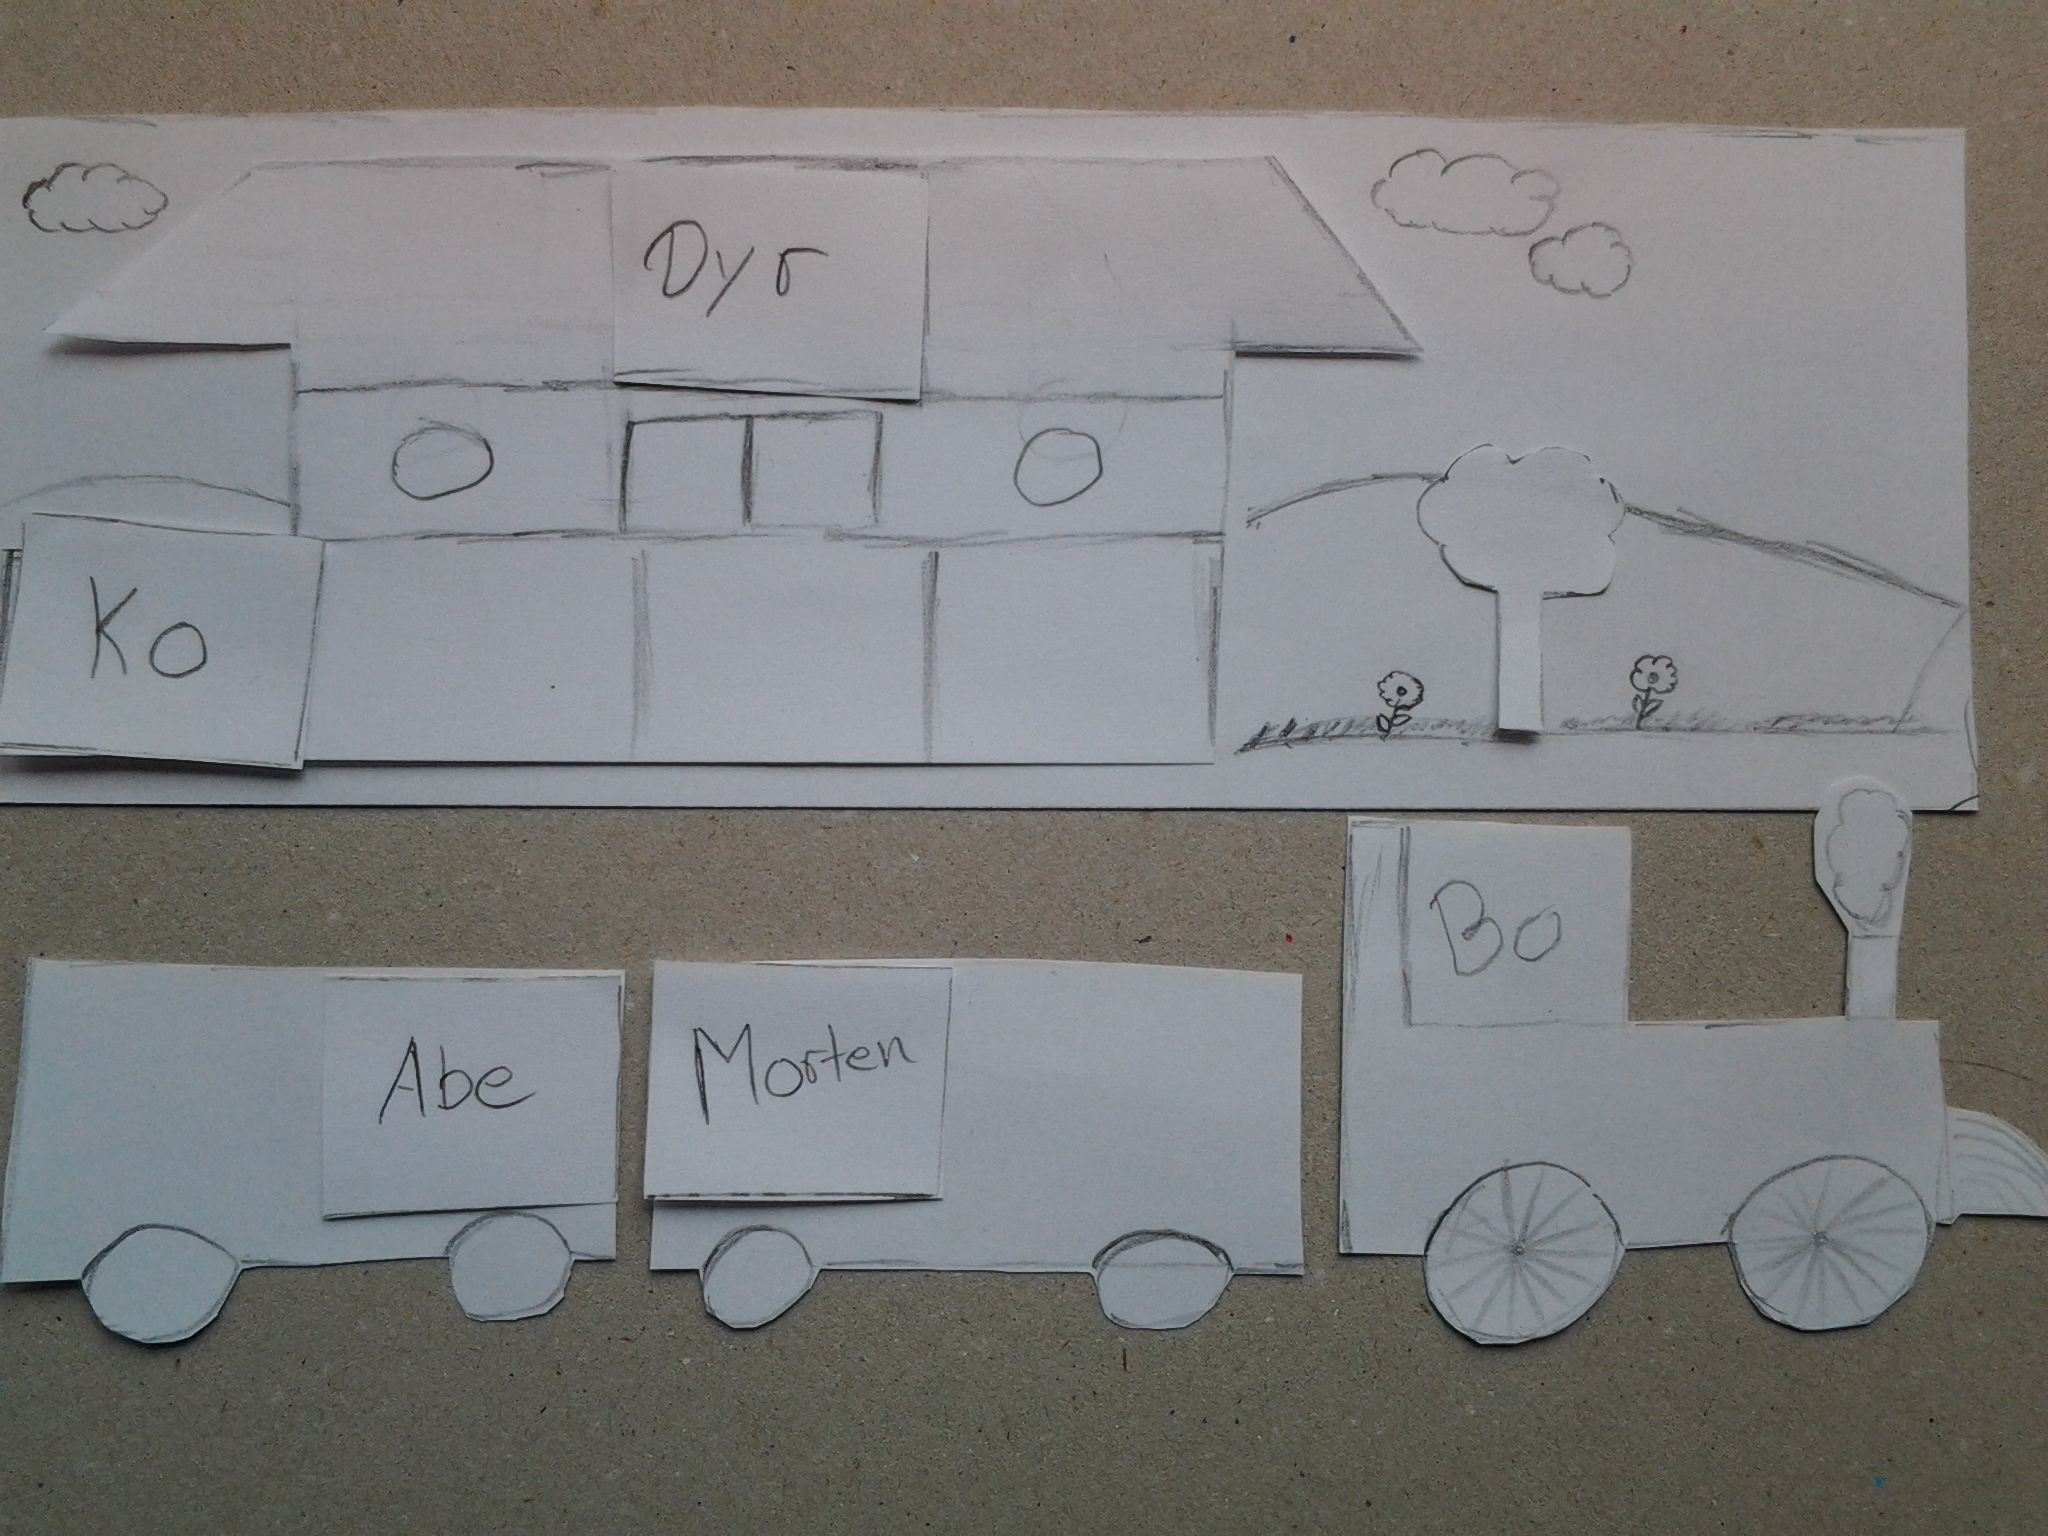
\includegraphics[width=0.9\linewidth]{img/screenshots/prototype1.jpg}%0.1 margin
\caption{The paper prototype}
\label{fig:paperprototype}
\end{figure}
\autoref{fig:paperprototype} shows the paper prototype we showed Tove at our first meeting. We explained the general game idea: by drag and dropping pictograms off the train to the correct station. She liked the idea and the interface, although she wished to see a button that would check if the correct pictograms was off the train, and start the train. She also mentioned that the game should not contain many different colors and sounds, since this would cause visual and audible noise for the child.	

\subsection*{Game Interface}
\begin{figure}[H]
\centering
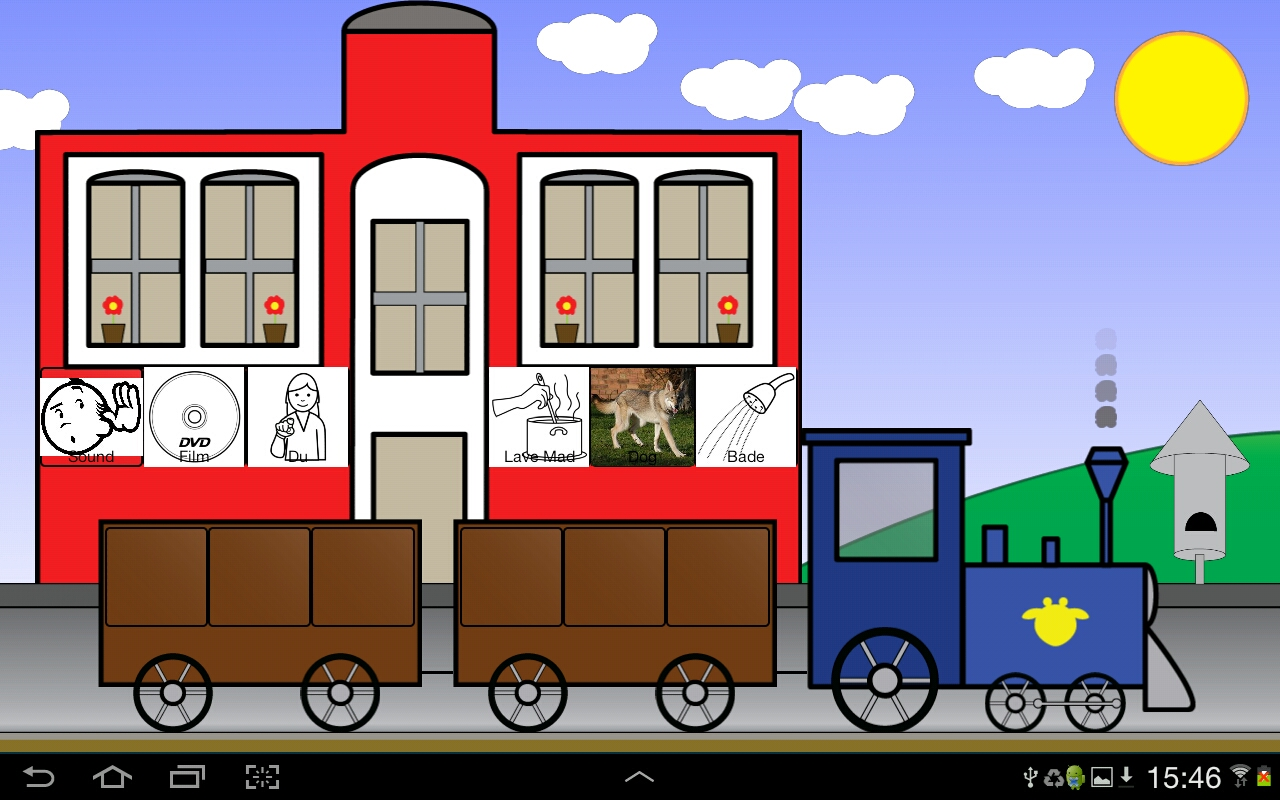
\includegraphics[width=0.9\linewidth]{img/screenshots/gamedesign1.jpg}%0.1 margin
\caption{The final result}
\label{fig:finalresult}
\end{figure}
During the project we sent screen shots of the game interface to Tove, to confirm that we were on the right track. For the most part she had not much to add, only small graphical adjustments to stations.
%hvis det endelig resultat, samt de ting som ikke noget at blive tilføjet.(Traindriver, click and autosnap, lyd på pictogrammer)